% !TEX root = ../agglo_clust_review.tex

\begin{minipage}[t]{\textwidth}
        \centering
        \begin{minipage}[t]{0.45\textwidth}
\centering
        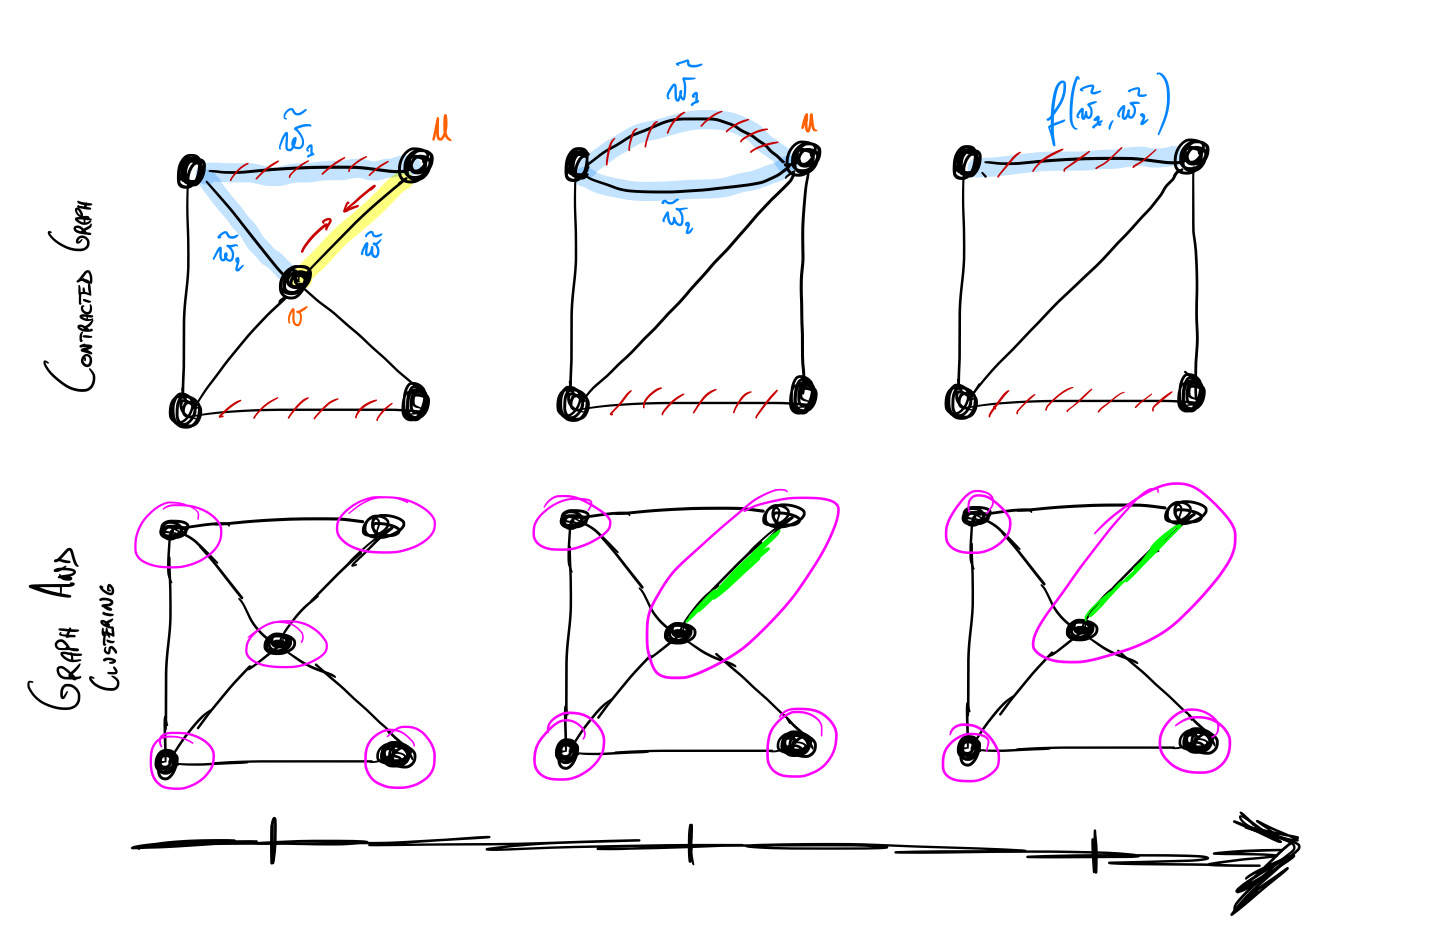
\includegraphics[width=\textwidth,trim=0.1in 0.4in 0.2in 0.2in,clip]{./figs/edge_contraction.png} % left bottom right top
\captionof{figure}{\small 
Example of edge contraction: the edge $e_{uv}$ is selected from priority queue; after nodes $u$ and $v$ are merged and $e_{uv}$ is deleted, there are two double edges $e_1$ and $e_2$ left in the graph...  
\label{fig:edge_contraction_and_contr_graph} }
    \end{minipage}\hspace{0.04\textwidth}
    \begin{minipage}[t]{0.45\textwidth}
        \centering
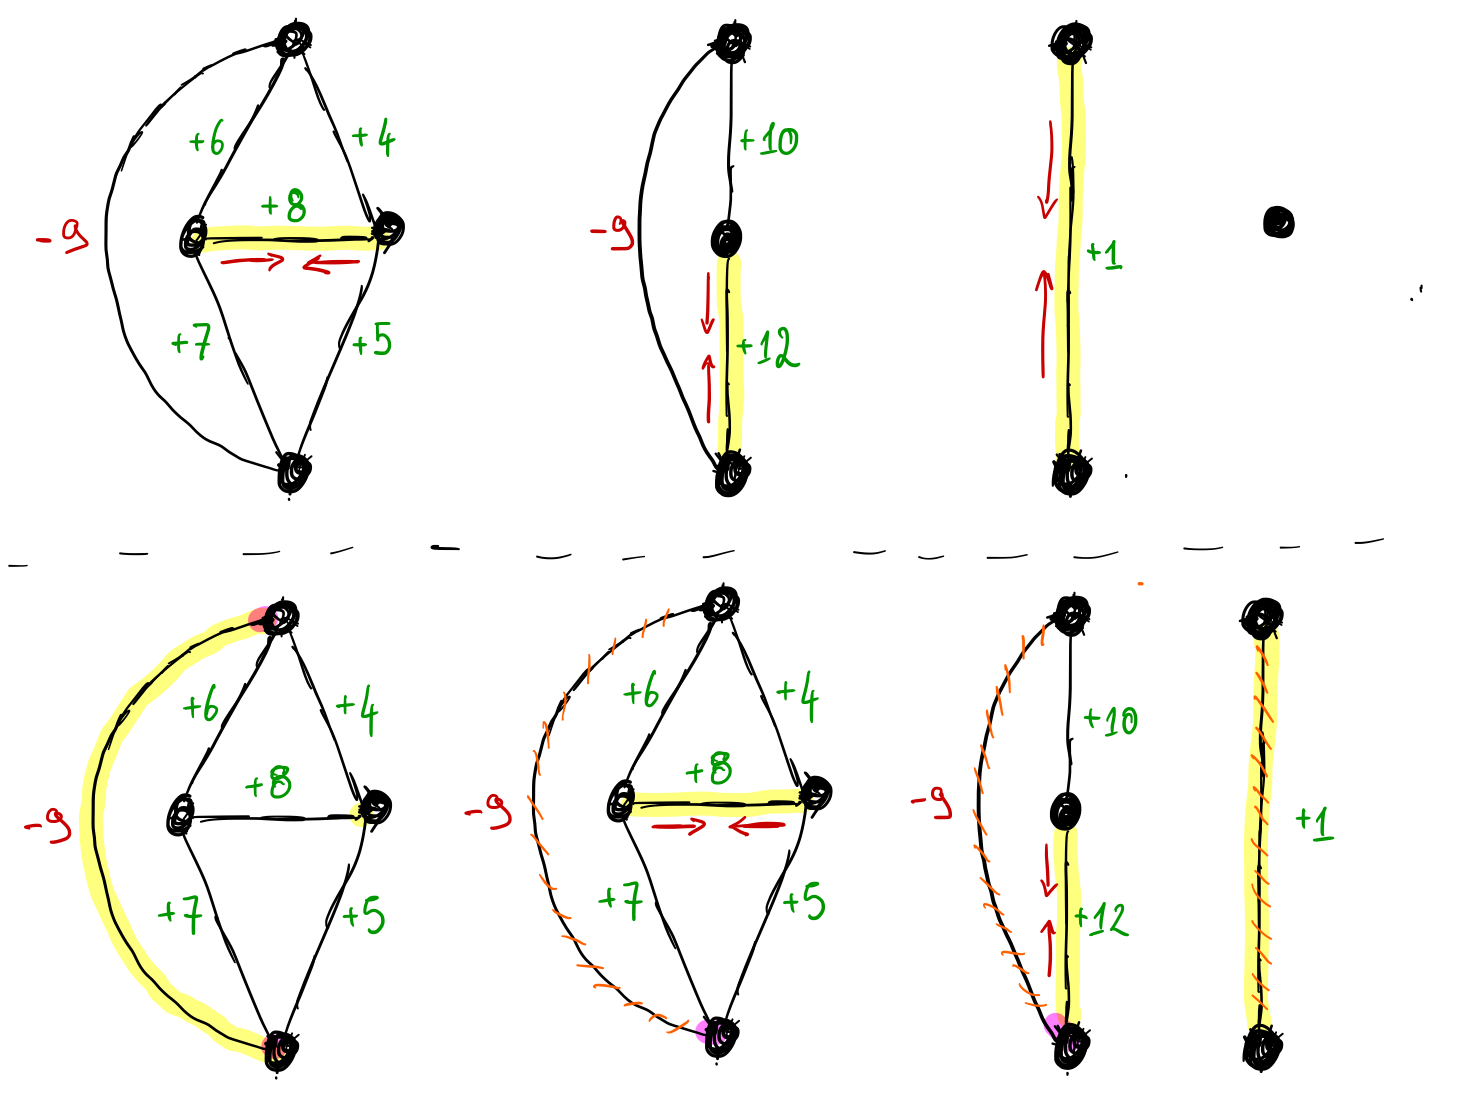
\includegraphics[width=0.8\textwidth,trim=0.in 0.in 0.in 0.in,clip]{./figs/cannot-lin-constraints.jpg}
\captionof{figure}{\small 
Example of agglomerative clustering on signed graph with and without cannot-link constraints...
\label{fig:algorithm_with_without_CLC}}
    \end{minipage}
\end{minipage}


\section{Unified Graph Agglomerative Clustering}
In this section we introduce the Unified Graph Agglomerative Clustering Algorithm (UGACA) that represents a simple generalized formalization of many agglomerative graph clustering algorithms. \UPDATE{It can be used to describe both unsigned clustering algorithms ingesting positive node similarities and signed clustering algorithms using attractive and repulsive cues.}\\
First, we define notation and the concept of cannot-link constraints. Then, we introduce the generalized algorithm and show \UPDATE{how it can be used to introduce several new agglomerative clustering algorithms for graphs with signed edge weights.}

\subsection{Signed graph formalism: edge contraction and cannot-link constraints} \label{sec:contr_graph_and_CLC}

\begin{itemize}
\item \TODO{First define clustering, then weights, costs} We consider the problem of clustering a simple graph $\mathcal{G}(V,E,w^+, w^-)$ with both attractive and repulsive edge attributes. The weight function $w^+: E \rightarrow \mathbb{R}^+$ associates a positive scalar attribute $w_e^+$ to each edge $e \in E$ representing a merge affinity: the higher this number, the higher the inclination of the two incident vertices to be assigned to the same cluster\footnote{Note that several formalisms defining unsigned weighted graphs associate to each edge a positive scalar that represents a metric or distance on the graph. In these formalisms, the \emph{lower} the edge weight, the higher the attraction between the two linked nodes, contrary to our definition of $w^+: E \rightarrow \mathbb{R}^+$.}. On the other hand, $w^-: E \rightarrow \mathbb{R}^+$ associates a split tendency $w_e^-$ to each edge: the higher this weight, the greater the desire of the incident vertices to be in different clusters.
Graphs that have only positive weights can be seen as special cases of the previously defined graph $\mathcal{G}(V,E,w^+,w^-)$, when $w^-_e=0$ for every $e \in E$.   

\item The set $\Pi$ is defined as a partition of the set of nodes $V$ into $K$ subsets if $V = \cup_{i=1}^K S_i $ and $S_i \cap S_j = \emptyset$ for every $i\neq j \in \{1, ..., K\}$. We call a partition $\Pi$ of $V$ a \emph{clustering} if every $S \in \Pi$ induces a connected subgraph (\emph{cluster}) of $\mathcal{G}$.
\item For any clustering $\Pi$ of $\mathcal{G}$, we define as $E^0_\Pi$ the set of edges linking nodes in the same cluster, and as $E_\Pi^1$ the complementary set of edges whose linked nodes belong to distinct clusters:

\begin{align}
E_\Pi^0 &= \{ uv \in E \,|\, \exists S \in \Pi : u \in S \, \text{and} \, v \in S \}, \\
E^1_\Pi &= E \setminus E^0_\Pi.
\end{align}

The set of edges $E_\Pi^1$ is known as the \emph{multicut} of $\mathcal{G}$ associated to the clustering $\Pi$. 
\item Often, graphs with both attractive and repulsive edge attributes are described in terms of a cost function $c: E \rightarrow \mathbb{R}$   The NP-hard multicut graph partition problem also called \emph{correlation clustering} \TODO{cits} amounts to finding a graph multicut $E^1_\Pi$ for which the sum of costs $c_e = w^-_e - w^+_e$  
for every edge e
\item Given a clustering $\Pi$ and a graph $\mathcal{G}(V,E,W)$, the interaction between two clusters $S_1, S_2 \in \Pi$ is usually defined in terms of a \emph{linkage criterion}, i.e. a function of all the edge weights connecting the two clusters:
\begin{equation} \label{eq:linkage_criterion_def}
\begin{gathered}
\mathcal{L}(S_1,S_2) = \mathcal{L}(\mathcal{W})\quad \\
   \text{where} \quad \mathcal{W} = \{ W(e_{uv})| u\in S_1, v\in S_2 \}.
\end{gathered}
\end{equation}

\item A cannot-link-constraint defines a mutual exclusion relationship between two nodes in the graph and is used to specify that the these two nodes should not be associated with the same cluster. (the alg. will introduce them dynamically)
\item The algorithm that we will present in the next section iteratively performs a sequence of \emph{edge contractions} on the original graph $\mathcal{G}(V,E,w^+, w^-)$.

\item define \emph{update rule} $f(c_1, c_2)$

\end{itemize}


\begin{algorithm}
  \caption{Unified Graph Agglomerative Clustering \TODO{adapt to width}}
   \hspace*{\algorithmicindent} \textbf{Inputs:} graph $\mathcal{G}(V,E,W)$; bool {\color{blue}\texttt{addCannotLink}}  \\
  \hspace*{\algorithmicindent} \textbf{Outputs:} Final clustering and contracted graph $\mathcal{G}'$\\
  \hspace*{\algorithmicindent} 
  \begin{algorithmic}[1]


    % \Procedure{SignedGraphEdgeContr}{{\color{blue}bool \emph{addConstraints}}}
      % \State $\mathcal{G}'\gets \mathcal{G}(V,E^+ \cup E^-)$ \Comment{Initialize the contracted graph}
      \State Initialize contracted graph $\mathcal{G}'$ from $\mathcal{G}$
      \State Initialize \texttt{canBeMerged}$[e] \gets$ \texttt{True} $\,\,\, \forall e\in E$
      \State Sort edges in priority queue (PQ) in desc. order of $|W_e|$ 
      \State
      \While{PQ is \textbf{not} empty}
        \State Pop edge $e_{uv}$ in $\mathcal{G}'$ with highest priority $|\tilde{w}|$
        \State
        \If{({\color{ForestGreen}\textbf{$\tilde{w} > 0$}}) \textbf{and} \texttt{canBeMerged}$[e_{uv}]$}
          
          % \State PQ, $\,E_\dagger,\,\, E' \gets$ \textsc{deleteDoubleEdges}($u,v$)
          
        %   \State Update costs of double edges;
        %   \State Propagate constrained flags of double edges;
          \State Contract $e_{uv}$ in $\mathcal{G}'$
          \For{every new pair of double edges $(e_1,e_2)$}
            \State Get priorities $\tilde{w}_1, \tilde{w}_2$ of $e_1,e_2$
            \State Use update rule $f(\tilde{w}_1,\tilde{w}_2)$ (see Table 1) to 
            \Statex \hspace{\algorithmicindent}\hspace{\algorithmicindent}\hspace{\algorithmicindent}\hspace{\algorithmicindent} update priority of $e_1$
            \State Delete $e_2$ from $\mathcal{G}'$
          \EndFor
          % \State  Replace double edges in $\mathcal{G}'$ with single edges
          % \Statex \hspace{\algorithmicindent}\hspace{\algorithmicindent}\hspace{\algorithmicindent} and update priorities
        \EndIf
        \State
        \If{({\color{red}\textbf{$\tilde{w} \leq 0$}}) \textbf{and} {\color{blue}\texttt{addCannotLink}}}
          % \State Flag $e_{uv}$ as MustNotLink
          \State \texttt{canBeMerged}$[e_{uv}] \gets$ \texttt{False}
        \EndIf
      \EndWhile


      % \For{$e  \in E$ in descending order of absolute costs $|W(e)|$}
      %   \If{({\color{ForestGreen}\textbf{$W(e) > 0$}}) \textbf{AND} (edge is not constrained)}
      %     \State Contract edge $e$ in the graph $\mathcal{G}'$;
      %     \State Update costs of double edges;
      %     \State Propagate constrained flags of double edges;
      %     % \For{every new double edge}
      %     %   \State Delete double edges
      %     %   \State Insert new one with updated cost
      %     % \EndFor
      %   \EndIf
      %   \If{({\color{red}\textbf{$W(e) \leq 0$}}) \textbf{AND} ({\color{blue}\emph{addConstraints}})}
      %     \State Flag edge $e$ as constrained
      %   \EndIf
      % \EndFor
      \State
      \State
      \Return $\mathcal{G}'$
      % \State


    % \EndProcedure

  \end{algorithmic}
  \label{main_alg}
\end{algorithm}


\subsection{The algorithm}

We now present our first contribution: a unified algorithm for agglomerative graph clustering that can describe in a simple general form many graph partitioning algorithms previously introduced in the literature \UPDATE{and highlights the existence of totally new algorithms}.

We consider a graph $\mathcal{G}(V,E,W)$ with associated signed edge weights, where each node initially represents one cluster.
The proposed graph partitioning algorithm is a general form of agglomerative clustering that outputs a final graph clustering $\Pi$ by progressively merging pairs of neighboring clusters. Intuitively, the algorithm starts by merging clusters with the strongest attractive interaction, corresponding to the highest positive weights in the graph, and it stops when the remaining clusters share only mutual repulsive interactions (see Fig. \hyperref[fig:intro_figure]{\ref*{fig:intro_figure}b} and \hyperref[fig:intro_figure]{\ref*{fig:intro_figure}c}). 

A second variant of the proposed algorithm also introduces cannot-link constraints between clusters during the agglomeration and stops when all the remaining clusters have been previously constrained (option \texttt{addCannotLink} in Algorithm \ref{main_alg}).


During the agglomerative process, the interaction between neighboring clusters is defined by the linkage criterion defined in Equation \ref{eq:linkage_criterion_def} and has to be properly updated and recomputed. 
An efficient way of implementing these updates can be achieved by using the presented edge contraction Algorithm \ref{main_alg}, which proceeds as follows.

Given an initial clustering $\Pi$ where each node of the original graph $\mathcal{G}$ represents its own cluster, the algorithm starts by initializing a contracted graph $\mathcal{G}'$ (see Definition \ref{def:contr_graph}) that will represent the clustering $\Pi$ at each iteration of the agglomeration. The algorithm then sorts all edges $e\in E$ by their absolute weight $|W(e)|$ in descending order in a priority queue, so that the most attractive and the most repulsive edges are processed first. It iteratively pops one edge $e_{uv}$ from priority queue and, depending on the value of the priority $\tilde{w}$ associated with $e_{uv}$, does the following: if the edge is attractive and $\tilde{w}>0$, then merge the connected nodes and perform an edge contraction of $e_{uv}$ in $\mathcal{G}'$ (see Sec. \ref{sec:contr_graph_and_CLC} and Fig. \ref{fig:edge_contraction_and_contr_graph}), provided that $e_{uv}$ was not previously flagged as a cannot-link constraint; for every new pair of double edges in $\mathcal{G}'$ update \UPDATE{their priorities} according to one of the update rules listed in Table \ref{tab:linkage-criteria} and update their cannot-link relationships (see example in Fig. \ref{fig:algorithm_with_without_CLC}b from step 3 to 4). If, on the other hand, the edge $e_{uv}$ is repulsive and $\tilde{w}\leq 0$, then flag it as a cannot-link constraint if and only if the algorithm input-option \texttt{addCannotLink} is true and mutual exclusion relationships should be enforced.

In the Supplementary material we provide a more detailed description of the algorithm (Sec. \ref{sec:detailed_algorithm}) and we also comment on its computational complexity (Sec. \ref{sec:complexity}).

 In the special case of an unsigned graph %$\mathcal{G}(V,E,W:E\rightarrow \mathbb{R}^+)$ 
 presenting strictly positive similarities between nodes, the algorithm returns only one single cluster as an output (see Fig. \hyperref[fig:intro_figure]{\ref*{fig:intro_figure}a}), \UPDATE{together with a merging tree representing the merging order and defining a hierarchy of clusters} \TODO{use def of merging process of contracted graph to define merging tree?}.

% \item Comment about must-not-link relations: they give high priority to the most confident repulsive edges {}


\begin{table*}
    \centering
    \begin{subtable}[t!]{\textwidth}\centering
        \begin{tabular}{r l || c | c | c}
            % \toprule\toprule
             & &  \multirow{3}{*}{\textbf{Unsigned graphs}}  & \multicolumn{2}{c}{\textbf{Signed graphs}}  \\        
            % \cmidrule(l{.15em}){4-5}
            % \cline{4-5}
            & & &  \multicolumn{2}{c}{\thead{Add Cannot-Link Constraints:}} \\        
           
            & & &  \thead{\textsc{No}} & \thead{\textsc{Yes}} \\        
            % \cmidrule[0.3em]{3-5}
            % \midrule[0.15em]
            \midrule\midrule
            Sum: & \thead[l]{$f(\tilde{w}_1,\tilde{w}_2) = \tilde{w}_1+\tilde{w}_2$} & \thead{Sum Linkage\\Hierarchical Clust.} & \thead{Greedy Additive \\ Edge Contraction \\\cite{levinkov2017comparative}} & \thead{Greedy \\Fixation \\\cite{levinkov2017comparative}} \\ \midrule
            
            \makecell[r]{Abs. \\ max:} & \thead[l]{
            $
            f(\tilde{w}_1,\tilde{w}_2) = \begin{cases} 
            \tilde{w}_1 & \text{if}\,\, |\tilde{w}_1|>|\tilde{w}_2|\\
            \tilde{w}_2 & \text{otherwise}
             \end{cases} 
            $}
               & \thead{Single Linkage\\Hierarchical Clust.\\ \cite{lance1967general}} & \thead{Mutex \\Watershed \\\cite{wolf2018mutex}} & \thead{Mutex \\Watershed \\\cite{wolf2018mutex}} \\ \midrule
            \makecell[r]{Mean:} & \thead[l]{$f(\tilde{w}_1,\tilde{w}_2) = \mathrm{wAvg}\{ \tilde{w}_1, \tilde{w}_2 \} $}                                 & \thead{ Average Linkage\\ Hierarchical Clust. \\(UPGMA) \cite{lance1967general}} & \thead{Average Linkage\\Signed Aggl. Clust. \\ (\textbf{NEW})} & \thead{\textbf{NEW}}\\ \midrule

            Max: & \thead[l]{$f(\tilde{w}_1,\tilde{w}_2) = \max \{ \tilde{w}_1, \tilde{w}_2 \}  $}                                 & \thead{Single Linkage\\Hierarchical Clust.\\ \cite{lance1967general}} & \thead{Single Linkage \\Signed Aggl. Clust. \\ (\textbf{NEW})} & \thead{\textbf{NEW}}\\ \midrule

            Min:& \thead[l]{$f(\tilde{w}_1,\tilde{w}_2) = \min \{ \tilde{w}_1, \tilde{w}_2 \}  $}                                 & \thead{Complete Linkage\\ Hierarchical Clust. \\ \cite{lance1967general}}  & \thead{Complete Linkage \\Signed Aggl. Clust. \\ (\textbf{NEW})} & \thead{\textbf{NEW}}



            
        \end{tabular}
        % \caption{Linkage criteria}
    \end{subtable} 
    \caption{The table lists all the algorithms that can be seen as special cases of the Generic Agglomerative Clustering \ref{main_alg} given a specific update rule $f(e_1,e_2)$ and a type of graph...}
    \label{tab:linkage-criteria}
\end{table*}


\subsection{Update rules and associated algorithms}
\begin{itemize}
\item In this section we will list some of the algorithms that can be described using the generalized Algorithm \ref{main_alg} presented above and we will introduce some new ones.
\item In Table \ref{tab:linkage-criteria} we collected the update rules that we tested and compared in this article. Later we will mention more of them that were proposed in the literature.
\item In the special case of unsigned graphs (Table \ref{tab:linkage-criteria} column 1), the UGAC algorithm becomes simply a version of hierarchical clustering with different linkage criteria depending on the chosen update rule. It outputs one single cluster and it also defines a hierarchy of clusters during the merging process that can be associated to \UPDATE{a merging tree/  the hierarchical clustering dendrogram}... \TODO{Problem: sum does not trivially define an ultra-metric-distance...}  
\item In the literature there have been already several methods using cannot-link constraints for agglomerative clustering algorithms \TODO{repetition from related work}: for example, \cite{malmberg2011generalized} used initially fixed mutual exclusion relationships, whereas \cite{levinkov2017comparative} introduced them dynamically in an edge contraction algorithm for signed graphs, named Greedy Fixation (Table \ref{tab:linkage-criteria} row 1, \emph{sum}). At the same time, they also proposed a version of it without cannot link constraints (Greedy Additive Edge Contraction) and they compared both with other greedy and local-search algorithms for solving the multicut/correlation clustering problem.
\item Dynamically introduced cannot-link constraints were also proposed by \cite{wolf2018mutex}, that... \TODO{brief MWS description as efficient implementation of this update rule}. In the Supplementary material we show that the algorithm they present can be seen as a special case of UGACA with absolute maximum update rule (Table \ref{tab:linkage-criteria} row 2 - \emph{absolute maximum}) and that adding or not cannot-link constraints does not change the final clustering.
\item On the other hand, the signed graph versions of UGACA with update rules \emph{arithmetic mean}, \emph{max} and \emph{min} (rows 3 to 5 in Table \ref{tab:linkage-criteria}) are new algorithms that were never mentioned in the literature, \UPDATE{especially those with cannot-link constraints}.
\item In this article, we test and run a comparison of the five types of update rule listed in Table \ref{tab:linkage-criteria} (i.e. \emph{sum}, \emph{absolute mac}, \emph{arithmetic mean}, \emph{max} and \emph{min}), since \UPDATE{they they are the most commonly used and the cheapest to compute}. Nevertheless, UGACA can be easily generalized to include even more complex rules. For instance, \cite{nunez2013machine} proposes a learned version of update rule where a neural network updates the edge weights depending on edge and node features; another really common choice is to introduce a weight regularization depending on the size of the linked nodes (\cite{felzenszwalb2004efficient} and \cite{kardoostsolving} (unpublished...??), Thorsten..); 
\cite{funke2018large} on the other hand accumulate statistics for each \UPDATE{boundary between clusters} by keeping a discrete histograms of the edge weights and then computes quantiles from it.
\end{itemize}


% \begin{table*}[t]
%     \centering
%     \begin{subtable}[t!]{0.98\textwidth}\centering
%         \begin{tabular}{c | c }
%             \toprule\toprule
%             \makecell{Algorithm name} & \makecell{Algorithm description and \\linkage criteria}    \\
%             \midrule\midrule

%             Weighted Arithmetic Mean (WPGMA) & \thead{Assign a weighting $\alpha_e \in \mathbb{R}^+$, $\forall e \in E$ \\ \\ Linkage criteria: $w_{\mathrm{new}} = \frac{\alpha_1 w_1 +\alpha_2 w_2}{\alpha_1 + \alpha_2} $}  \\ \midrule
            
%             \makecell{Felzenszwalb Efficient \\Graph-based Image Segmentation \cite{felzenszwalb2004efficient}}  & \thead{Initially all edges have positive weights }  \\ \midrule

%             \makecell{Quantile Agglomeration Clustering (...?)}  & \thead{...}  \\ \midrule

%             \makecell{Graph-based active learning \\of agglomeration (GALA) \cite{nunez2013machine}}  & \thead{Assign set of edge features $\phi^{\mathrm{I}}_e$ and \\node features $\phi^{\mathrm{II}}_u$, $\forall u \in V$, $\forall e \in E$. \\ \\ A classifier $f$ with parameters $\theta$ predicts and updates\\ the cost of an edge: $w_e = f(\phi^{\mathrm{I}}_e, \phi^{\mathrm{II}}_u, \phi^{\mathrm{II}}_v; \theta)$, $\forall e_{uv} \in E$} \\ \midrule

%             % \makecell{$w_{\mathrm{new}}=w_{\tilde{e}}$,$\,
%             % \,$ where $\tilde{e}=\mathrm{arg}\max_{e\in \{e_{1},e_{2}\}} \left|w_e\right|$  }  & \thead{Mutex Watershed \cite{wolf2018mutex}} & \thead{Mutex Watershed \cite{wolf2018mutex}} \\ \midrule

%             % Arithmetic mean: $w_{\mathrm{new}} = (w_1+w_2) / 2 $                                 & \thead{Hierarchical Clustering \\ with Average Linkage (UPGMA)} & \thead{\textbf{NEW}}\\ \midrule

%             % Maximum: $w_{\mathrm{new}} = \max \{ w_1, w_2 \}  $                                 & \thead{Hierarchical Clustering \\ with Single Linkage} & \thead{\textbf{NEW}}\\ \midrule

%             % Minimum: $w_{\mathrm{new}} = \min \{ w_1, w_2 \}  $                                 & \thead{Hierarchical Clustering \\ with Complete Linkage} & \thead{\textbf{NEW}}



            
%         \end{tabular}
%         % \caption{Linkage criteria}
%         \label{tab:linkage-criteria}
%     \end{subtable} 
%     \caption{Linkage criteria 2}
% \end{table*}






